\section{Aufbau und Generierung der Irradiance Map} % (fold)
\label{sec:aufbau_und_generierung_der_irradiance_map}

	Lorem ipsum dolor sit amet, consectetur adipisicing elit, sed do eiusmod
	tempor incididunt ut labore et dolore magna aliqua. Ut enim ad minim veniam,
	quis nostrud exercitation ullamco laboris nisi ut aliquip ex ea commodo
	consequat. Duis aute irure dolor in reprehenderit in voluptate velit esse
	cillum dolore eu fugiat nulla pariatur. Excepteur sint occaecat cupidatat non
	proident, sunt in culpa qui officia deserunt mollit anim id est laborum.

	\begin{figure}[h]
		\begin{subfigure}[b]{0.33\textwidth}
			\center
			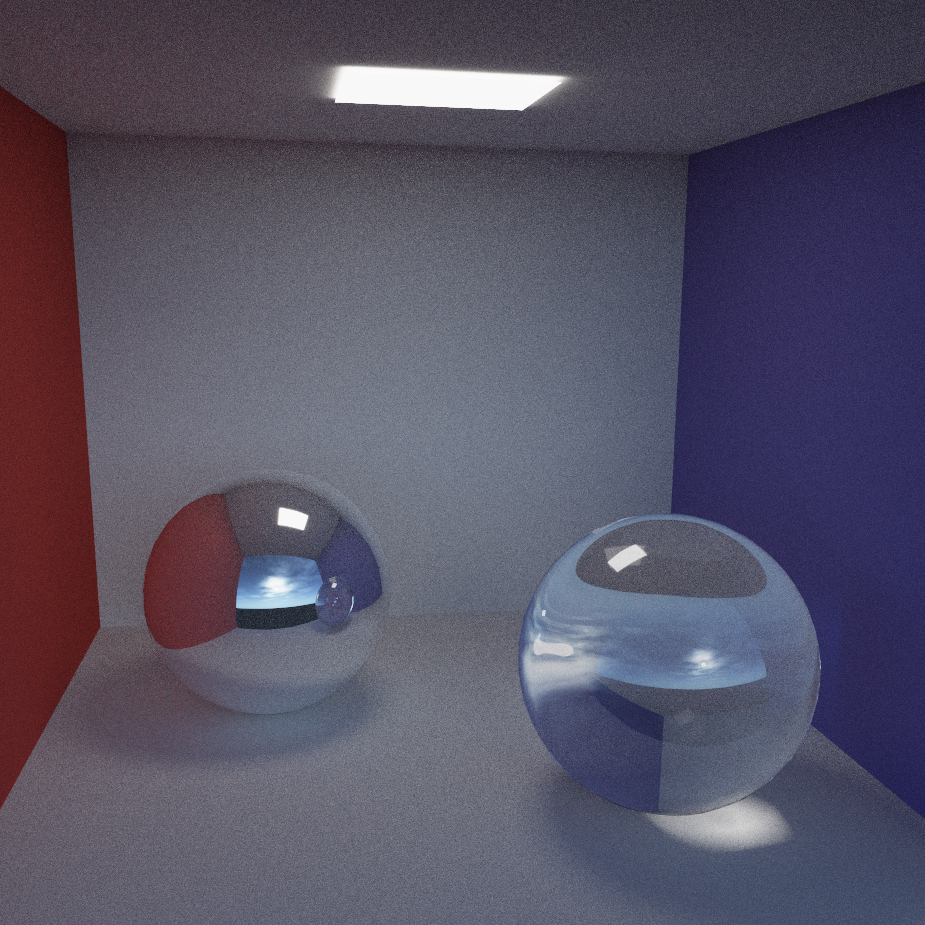
\includegraphics[width=0.95\textwidth]{pic/irrmap-cornell-ref.png}
			\caption{Path Tracing}
		\end{subfigure}
		\begin{subfigure}[b]{0.33\textwidth}
			\center
			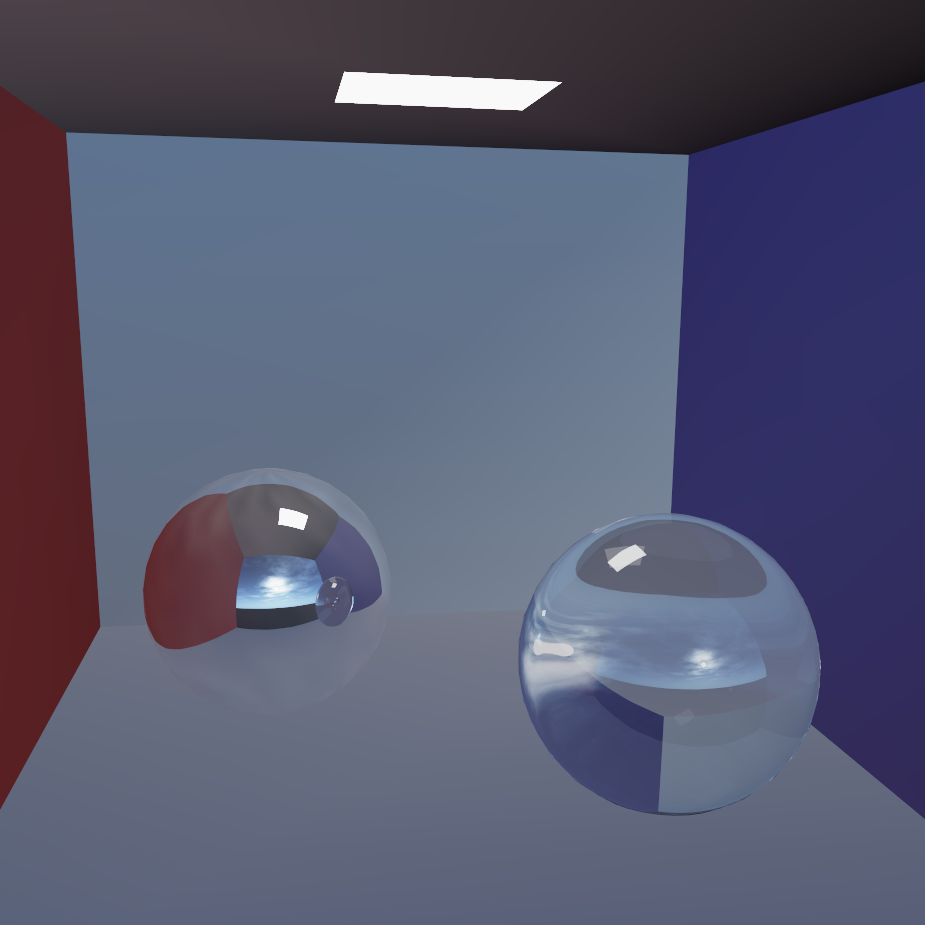
\includegraphics[width=0.95\textwidth]{pic/irrmap-cornell-vmap.png}
			\caption{Vertex Lighting}
		\end{subfigure}
		\begin{subfigure}[b]{0.33\textwidth}
			\center
			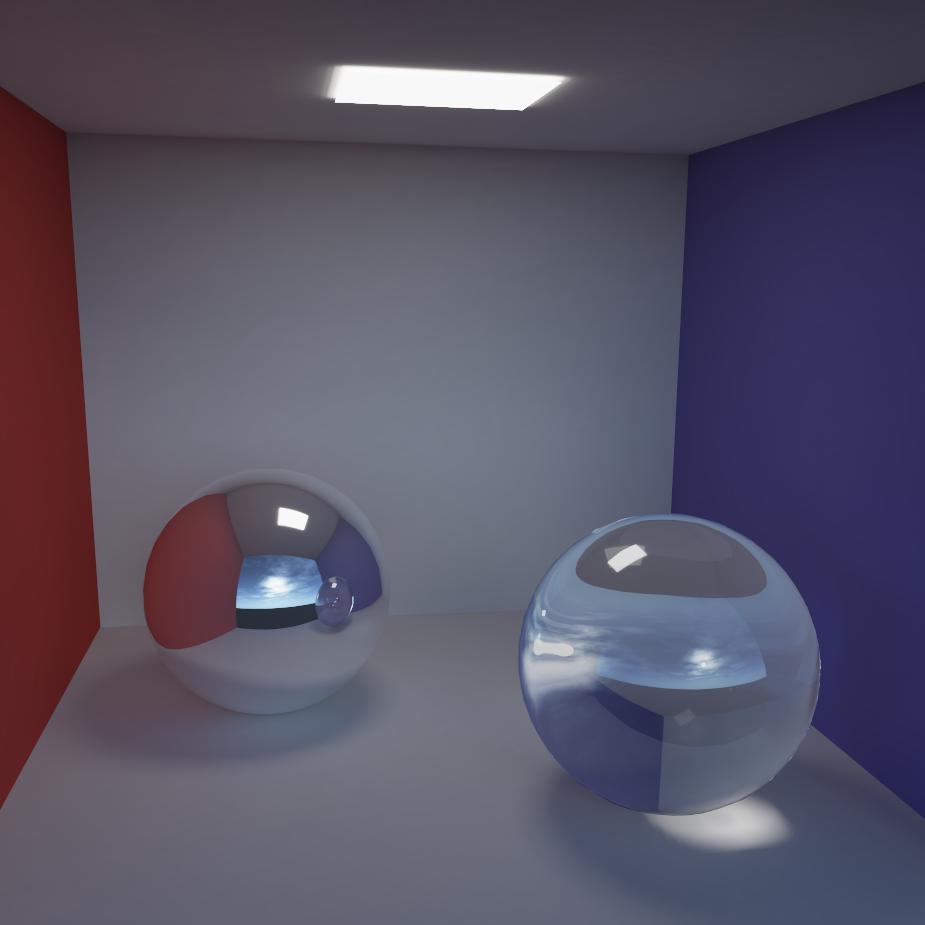
\includegraphics[width=0.95\textwidth]{pic/irrmap-cornell-irrmap.png}
			\caption{Irradiance Map}
		\end{subfigure}
		\caption[Irradiance-Map anhand der \enquote{Cornell Box}-Szene]{Die Bilder zeigen die Standardabweichungen der \enquote{Cornell Box}-Szene aus Abbildung \ref{fig:irr-est-rc-shaderball} entsprechend der Benennung aus Abbildung \ref{fig:irr-est-rc-dragon}. Vor allem Bereiche, die schwach von außen beleuchtet werden oder in Nischen liegen, weisen einen erhöhten Fehler auf. Die regelmäßigen Artefakte entstehen durch geringe Auflösung der Mesh in diesen Bereichen.}
		\label{fig:irr-map-cornell}
	\end{figure}

% section aufbau_und_generierung_der_irradiance_map (end)